\newpage
\section{Code implementation}
\subsection*{Machine learning implementation}

The machine learning analysis was written with Keras\cite{chollet2015keras} using the Tensorflow api\cite{tensorflow2015-whitepaper} . 
The machine learning structure was written using a functional structure\footnote{Functional structure uses a function call for layers, i.e for layers a,b, then b(a) will connect the two layers, and equals a sequential link a $\to$ b. This allows for more flexible structures. More on the functional api can be found \href{https://www.tensorflow.org/guide/keras/functional}{here}.}.
In practise, this model could just as well have been written as a Sequential model\footnote{Sequential structure adds layers in sequence, i.e for layers a, b, c we have that a $\to$ b $\to$ c, with a strict structure. This allows for more organized code. More on sequential models can be found \href{https://www.tensorflow.org/guide/keras/sequential_model}{here}.}, 
but at a cost of flexibility and lack of potential non-linear structure in the architecture. The code consists of one general class for
 the autoencoder, where the different testing cases are different classes inheriting from the parent class.\par



\subsection*{Construction of a neural network in Tensorflow}

Using the functional structure, a general neural network in the Tensorflow API can be constructed as shown below. 
\begin{lstlisting}[language=Python, style=pythonstyle, label={code:python_func_example_general}]
import tensorflow as tf


inputs = tf.keras.layers.Input(shape=data_shape, name="input")

# First hidden layer
First_layer = tf.keras.layers.Dense(
    units=30,
    activation="relu"
)(inputs)

# Second hidden layer
Second_layer = tf.keras.layers.Dense(
    units=45, 
    activation="relu"
)(First_layer)

# Second hidden layer
output_layer = tf.keras.layers.Dense(
    units=1, 
    activation="sigmoid"
)(Second_layer)


# Model definition
nn_model = tf.keras.Model(inputs, output_layer, name="nn_model")

hp_learning_rate = 0.0015
optimizer = tf.keras.optimizers.Adam(hp_learning_rate)
nn_model.compile(loss="mse", optimizer=optimizer, metrics=["mse"]) 
\end{lstlisting}
The neural network here contains one input layer, two hidden layers, and an output layer. The choice of nodes and activation functions are 
arbitrary here as the use case has not been defined. Note that this is exactly the same as the previous example, but using the sequential structure.


\begin{lstlisting}[language=Python, style=pythonstyle, label={code:python_seq_example}]
import tensorflow as tf

nn_model = tf.keras.Sequential(
    [
        tf.keras.layers.Dense(30, activation="relu", input_shape=data_shape),
        tf.keras.layers.Dense(45, activation="relu"),
        tf.keras.layers.Dense(1, activation="sigmoid"),
    ]
)

hp_learning_rate = 0.0015
optimizer = tf.keras.optimizers.Adam(hp_learning_rate)
nn_model.compile(loss="mse", optimizer=optimizer, metrics=["mse"]) 
\end{lstlisting}


\subsection*{Data handling python side}


%Optimizing \cite{ADAM:opti}, \par 
%Plotting \cite{Hunter:2007}, \par
%More plotting  \cite{Waskom2021}, \par

\subsection*{Implementation of the RMM matrix}
An example of the RMM matrices used in this thesis is shown in figure \ref{fig:rmm_singular_events} below:


\begin{figure}[h!]
    \centering
    \begin{subfigure}{.8\textwidth}
        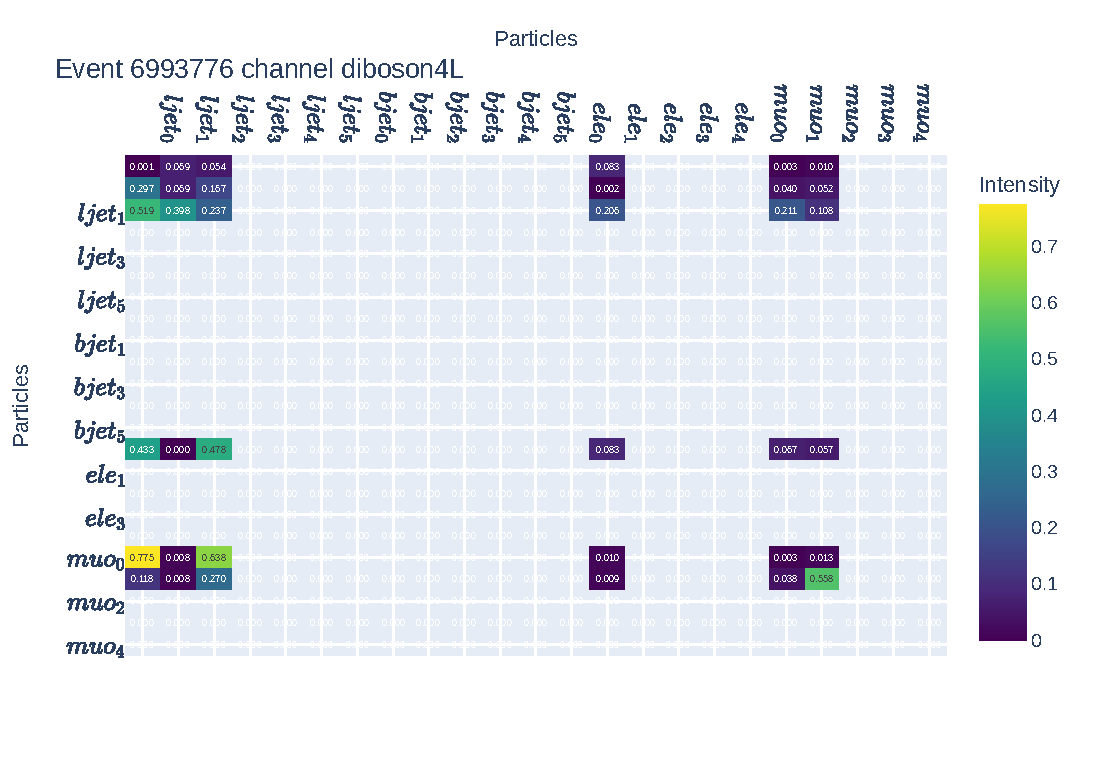
\includegraphics[width=\textwidth]{Figures/rmms/rmm_event_6993776_diboson4L.pdf}
        \caption{RMM matrix for event number 6993776 from the MonteCarlo diboson4L sample. Each feature is scaled based on a fit for that feature for 
        all events in the training set ($\approx 80\%$ of total MC). This sample contains two ljets, one electron and two muons.}
        \label{fig:rmm_zee_event}
    \end{subfigure}
    \hfill
    \begin{subfigure}{.8\textwidth}
        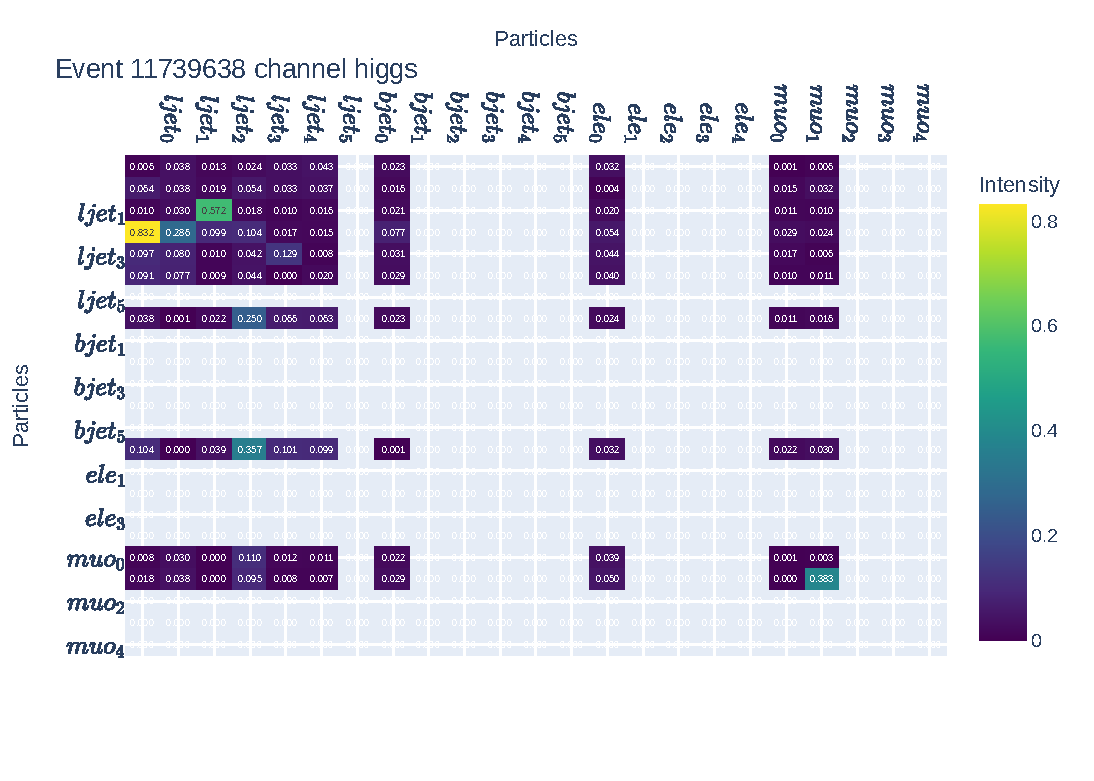
\includegraphics[width=\textwidth]{Figures/rmms/rmm_event_11739638_higgs.pdf}
        \caption{ RMM matrix for event number 11739638 from the MonteCarlo Higgs sample. Each feature is scaled based on a fit for that feature for 
        all events in the training set ($\approx 80\%$ of total MC). This sample contains five ljets, one bjet, one electron and two muons. }
        \label{fig:rmm_higgs_event}
    \end{subfigure}
    \hfill        
    \caption[Single event RMM plot]{Note here that the y axis for the RMM's lack every other label, due to lack of space in the y axis of the plot. If looked more closely upon, one can see that 
    each figure have all RMM cells, just that the labels, which are identical to the x axis label, only show every other. Note also here that the labels only tell which particle are used for that row/column, i.e 
    in figure \ref{fig:rmm_higgs_event} in row 0 column 3 we have the invariant mass of the first and second ljet. The RMM plots were created using 
    Plotly\cite{plotly}. }
    \label{fig:rmm_singular_events}
\end{figure}

In figure \ref{fig:rmm_singular_events} we see two RMM matrices created from two different channels in the MonteCarlo samples. 
This RMM is of type T4N5\footnote{T4 $\to$ 4 particle types: bjets, ljets, electrons and muons. N5 $\to$ 5 particles per 
particle type. Note here that we have 5 particles only for the leptons, and 6 particles for each of the types of jets.}. 
 For easier interpretability, the gray area corresponds to a missing value, leading to so called "islands" in the RMM matrix.



\subsubsection*{Setup for 3 lepton dataset}
The 3 lepton dataset is about 96 Giga bytes of data when implementing the RMM structure for 6 b- and ljets, 5 electrons and 5 muons. The dataset 
is converted from a ROOT RDataframe to a Pandas dataframe\cite{reback2020pandas} for further preprocessing. Having added the channel column in 
the dataset\footnote{This column would in a fully supervised setting be used as a target vector, but in this thesis it will only be used for legends in
histograms and to index out certain channels in the validation and training set. }, the channel categories, weights, missing transverse energy and 
trilepton mass\footnote{Invariant mass of three leptons. This is assured to exist from event selection in the 3 lepton dataset.} as well as the RMM structure are divided into 
a training and validation/test set in an 80-20 split. This was done using the "$.fit\_transform()$" and "$.transform()$" functions from the 
Scikit-learn library\cite{scikit-learn}. The training and validation/test set are then converted to numpy arrays\cite{harris2020array} for faster 
loading and easier indexing, and saved as ".npy" files. This allows for faster reuse of the arrays. 

\subsubsection*{Setup via iterative training for 2 lepton dataset}
The two lepton dataset contains about 1.5 - 2 Terra bytes of data when implementing the RMM structure for 6 
b- and ljets, 5 electrons and 5 muons, as for the 3 lepton dataset. This is too much to hold in memory at the same time, thus it had to 
be split into several smaller datasets, called megasets. Below is a figure visualizing the structure used. 

\begin{figure}[h!]
    \centering
    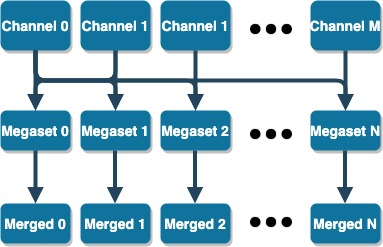
\includegraphics[width=0.6\linewidth]{Figures/2lep_config/megaset_struct.jpeg}
    \caption[Megaset structure diagram]{Megaset structure for the 2lep dataset. This figure generalises to M channels, and N megasets. The more you increase the number of megasets, 
    the smaller each megaset will be in bytesize, but in order to keep the SM MC distribution, it is not recommended to make too small sets.  }
    \label{fig:2lep_struct}
\end{figure}




In figure \ref{fig:2lep_struct} we see a generalized dividing structure. In the case of this thesis, each channel was divided into 10 equal parts, 
and stored in their respective folder. Pandas is not built for very large datasets, not running in a parallalized way. To handle this, the library
Polars
\footnote{Polars uses all available cores on the system and has excellent memory handling capability, see \href{https://pola-rs.github.io/polars-book/user-guide/}{Polars User Guide}}
\cite{ritchie_vink_2023_7744139} was used instead. When all channels were split, a merging was done combining all the channels in a given 
megaset to a separate dataset. The selection of events from each channel was done randomly, 
which is important, as we want to the best of our ability keep the distribution signature of the entire dataset in each megaset. If not, the model will 
be biased towards those datasets with the most events. Once each of the megasets where merged, the training could begin in an iterative fashion. Because
Tensorflow is statically compiled, you cannot call the fit function over and over again. Instead, the weights trained based on one megaset is stored and 
reloaded into a new model, thus the weights are still trained on the entire set, but in a batch like manner. 

\begin{lstlisting}[language=Python, style=pythonstyle, label={code:megabatch_training}]
for megaset in range(self.totmegasets):
    
    #* Load model 
    if SMALL:
        self.AE_model = nn_model.getModel()
    else:
        self.AE_model = nn_model.getModelBig()
    
    if megaset != 0:
        self.AE_model.load_weights('./checkpoints/Megabatch_checkpoint')
        
        
    #* Run Training
    with tf.device("/GPU:0"):

        tf.config.optimizer.set_jit("autoclustering")

        self.AE_model.fit(
            xtrain,
            xtrain,
            epochs=self.epochs,
            batch_size=self.b_size,
            validation_data=(xval, xval),
            sample_weight=x_train_weights,
        )
        
    
    self.AE_model.save_weights('./checkpoints/Megabatch_checkpoint')

\end{lstlisting}


